\documentclass{standalone}
\usepackage{tikz}
\usetikzlibrary{patterns, positioning}
\usepackage[sfdefault]{ClearSans} %% option 'sfdefault' activates Clear Sans as the default text font
\usepackage[T1]{fontenc}

\begin{document}
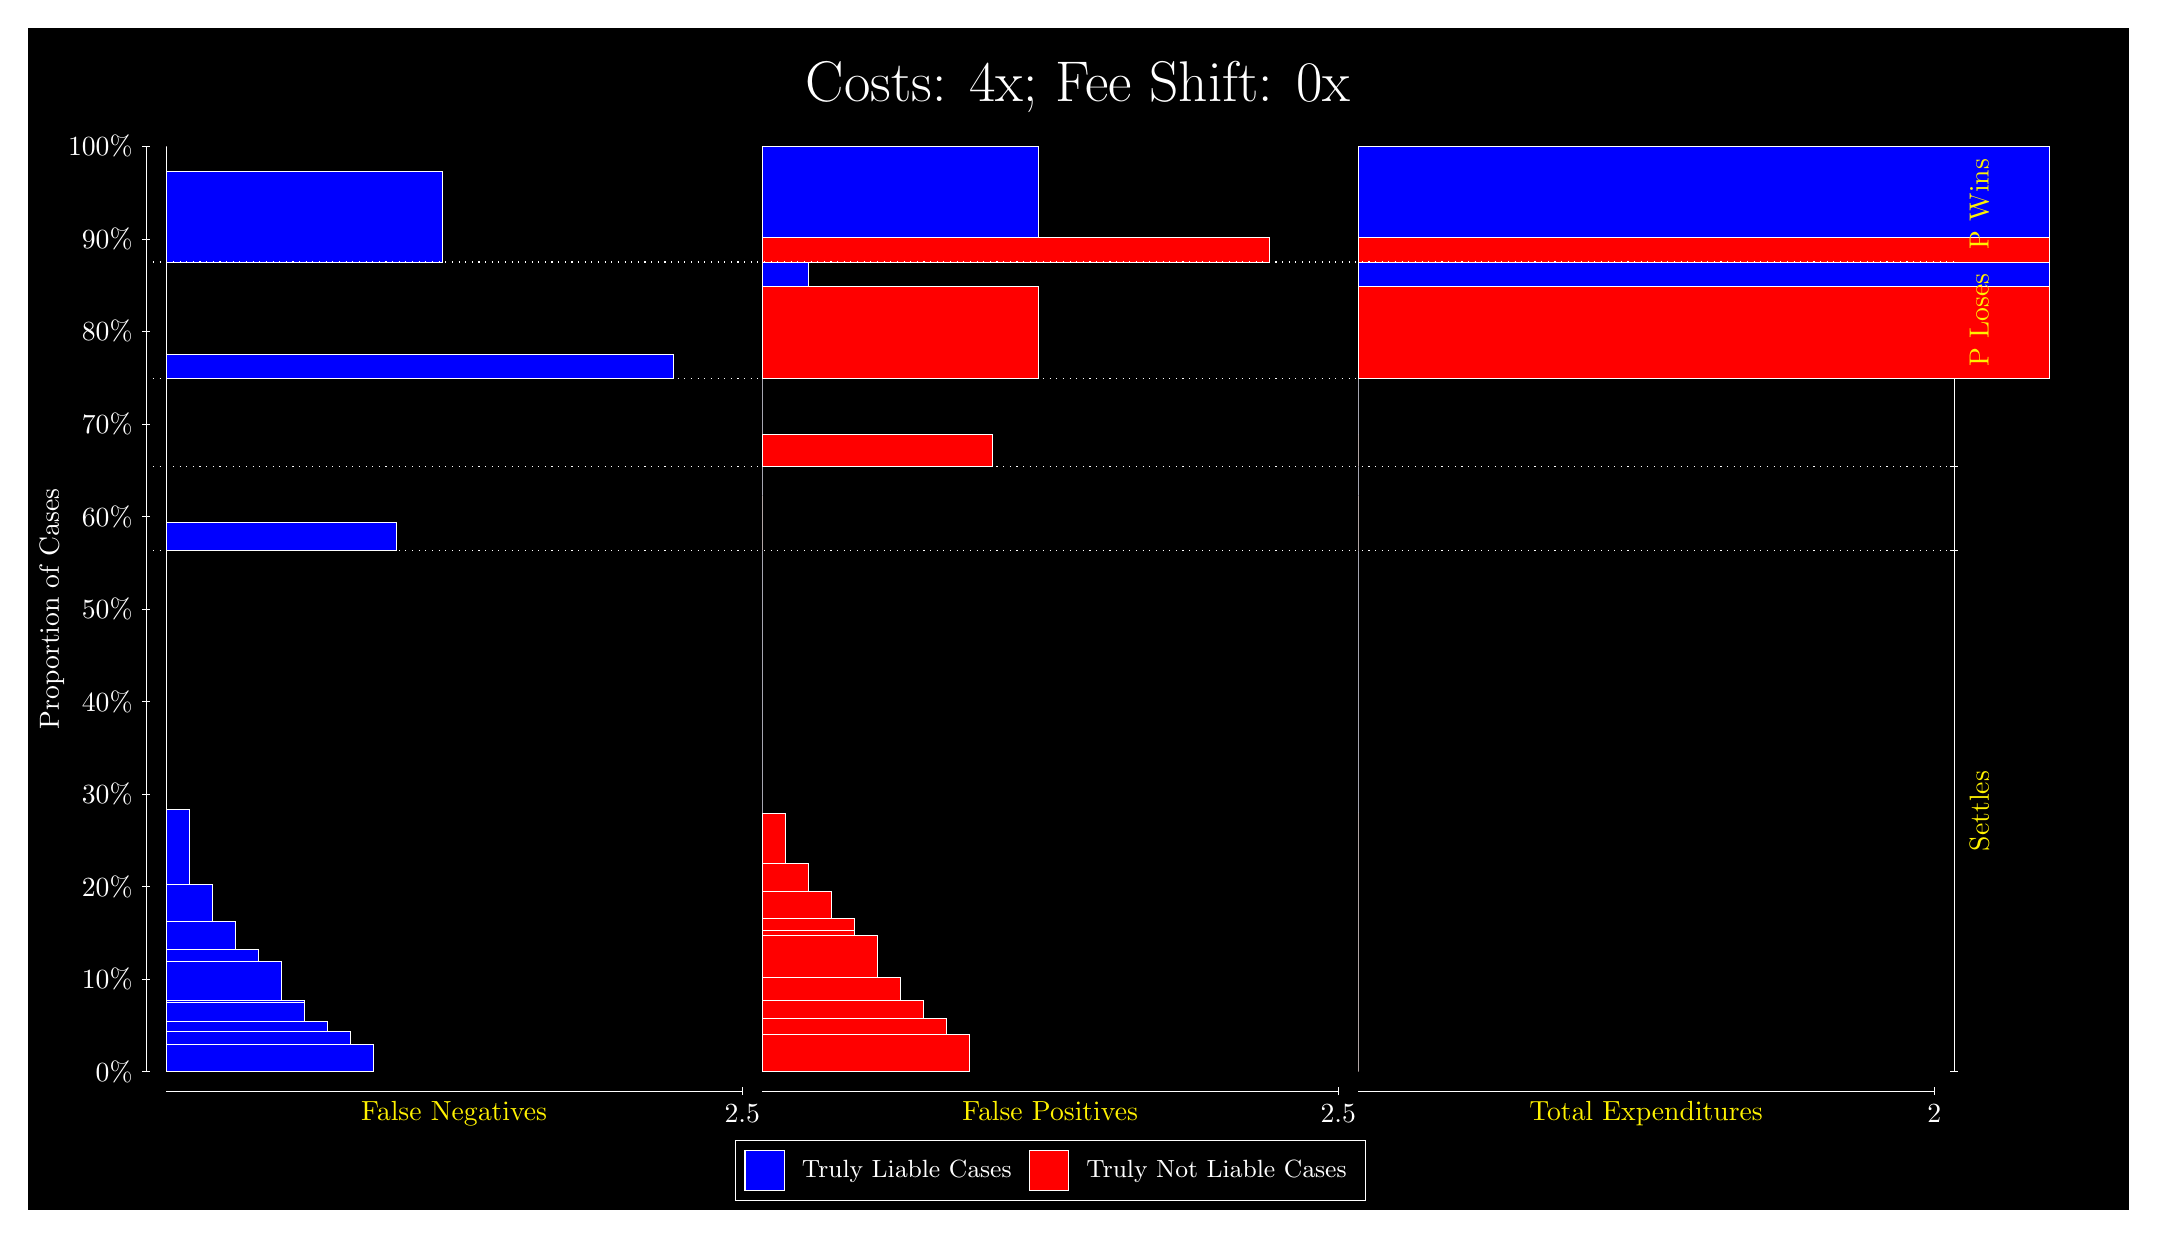
\begin{tikzpicture}
\draw[fill=black] (0,0) rectangle (26.667,15);
\draw[text=white] (0,13.5) rectangle (26.667,15) node[midway] {\huge Costs: 4x; Fee Shift: 0x};
\draw[white, very thin] (1.5,1.75) -- (1.5,13.5);
\node[rotate=90, text=white, anchor=center] at (0.3, 7.625) {Proportion of Cases};
\draw[white, very thin] (1.45,1.75) -- (1.55,1.75);
\node[text=white, anchor=east] at (1.45, 1.75) {0\%};
\draw[white, very thin] (1.45,2.925) -- (1.55,2.925);
\node[text=white, anchor=east] at (1.45, 2.925) {10\%};
\draw[white, very thin] (1.45,4.1) -- (1.55,4.1);
\node[text=white, anchor=east] at (1.45, 4.1) {20\%};
\draw[white, very thin] (1.45,5.275) -- (1.55,5.275);
\node[text=white, anchor=east] at (1.45, 5.275) {30\%};
\draw[white, very thin] (1.45,6.45) -- (1.55,6.45);
\node[text=white, anchor=east] at (1.45, 6.45) {40\%};
\draw[white, very thin] (1.45,7.625) -- (1.55,7.625);
\node[text=white, anchor=east] at (1.45, 7.625) {50\%};
\draw[white, very thin] (1.45,8.8) -- (1.55,8.8);
\node[text=white, anchor=east] at (1.45, 8.8) {60\%};
\draw[white, very thin] (1.45,9.975) -- (1.55,9.975);
\node[text=white, anchor=east] at (1.45, 9.975) {70\%};
\draw[white, very thin] (1.45,11.15) -- (1.55,11.15);
\node[text=white, anchor=east] at (1.45, 11.15) {80\%};
\draw[white, very thin] (1.45,12.325) -- (1.55,12.325);
\node[text=white, anchor=east] at (1.45, 12.325) {90\%};
\draw[white, very thin] (1.45,13.5) -- (1.55,13.5);
\node[text=white, anchor=east] at (1.45, 13.5) {100\%};

\draw[white, very thin] (24.457,1.75) -- (24.457,13.5);
\draw[white, very thin] (24.407,1.75) -- (24.507,1.75);
\node[anchor=west] at (24.407, 1.75) {};
\draw[white, very thin] (24.407,8.3677) -- (24.507,8.3677);
\node[anchor=west] at (24.407, 8.3677) {};
\draw[white, very thin] (24.407,9.4315) -- (24.507,9.4315);
\node[anchor=west] at (24.407, 9.4315) {};
\draw[white, very thin] (24.407,10.553) -- (24.507,10.553);
\node[anchor=west] at (24.407, 10.553) {};
\draw[white, very thin] (24.407,12.031) -- (24.507,12.031);
\node[anchor=west] at (24.407, 12.031) {};
\draw[white, very thin] (24.407,13.5) -- (24.507,13.5);
\node[anchor=west] at (24.407, 13.5) {};

\draw[white, very thin, fill=blue] (1.75,1.75) rectangle (4.3848,2.0961);
\draw[white, very thin, fill=blue] (1.75,2.0961) rectangle (4.092,2.2553);
\draw[white, very thin, fill=blue] (1.75,2.2553) rectangle (3.7993,2.3852);
\draw[white, very thin, fill=blue] (1.75,2.3852) rectangle (3.5065,2.6266);
\draw[white, very thin, fill=blue] (1.75,2.6266) rectangle (3.5065,2.6496);
\draw[white, very thin, fill=blue] (1.75,2.6496) rectangle (3.2138,3.1529);
\draw[white, very thin, fill=blue] (1.75,3.1529) rectangle (2.921,3.3022);
\draw[white, very thin, fill=blue] (1.75,3.3022) rectangle (2.6283,3.6551);
\draw[white, very thin, fill=blue] (1.75,3.6551) rectangle (2.3355,4.1219);
\draw[white, very thin, fill=blue] (1.75,4.1219) rectangle (2.0428,5.0838);
\draw[white, very thin, fill=red] (1.75,5.0838) rectangle (1.75,8.3677);
\draw[white, very thin, fill=blue] (1.75,8.3677) rectangle (4.6775,8.7316);
\draw[white, very thin, fill=red] (1.75,8.7316) rectangle (1.75,9.4315);
\draw[white, very thin, fill=red] (1.75,9.4315) rectangle (1.75,9.8446);
\draw[white, very thin, fill=blue] (1.75,9.8446) rectangle (1.75,10.553);
\draw[white, very thin, fill=blue] (1.75,10.553) rectangle (8.1906,10.864);
\draw[white, very thin, fill=red] (1.75,10.864) rectangle (1.75,12.031);
\draw[white, very thin, fill=blue] (1.75,12.031) rectangle (5.2631,13.189);
\draw[white, very thin, fill=red] (1.75,13.189) rectangle (1.75,13.5);
\draw[white, very thin, fill=red] (9.3189,1.75) rectangle (11.954,2.2272);
\draw[white, very thin, fill=red] (9.3189,2.2272) rectangle (11.661,2.4313);
\draw[white, very thin, fill=red] (9.3189,2.4313) rectangle (11.368,2.6591);
\draw[white, very thin, fill=red] (9.3189,2.6591) rectangle (11.075,2.9423);
\draw[white, very thin, fill=red] (9.3189,2.9423) rectangle (10.783,3.4764);
\draw[white, very thin, fill=red] (9.3189,3.4764) rectangle (10.49,3.5481);
\draw[white, very thin, fill=red] (9.3189,3.5481) rectangle (10.49,3.7014);
\draw[white, very thin, fill=red] (9.3189,3.7014) rectangle (10.197,4.0377);
\draw[white, very thin, fill=red] (9.3189,4.0377) rectangle (9.9044,4.3975);
\draw[white, very thin, fill=red] (9.3189,4.3975) rectangle (9.6116,5.0339);
\draw[white, very thin, fill=blue] (9.3189,5.0339) rectangle (9.3189,8.3677);
\draw[white, very thin, fill=red] (9.3189,8.3677) rectangle (9.3189,9.0677);
\draw[white, very thin, fill=blue] (9.3189,9.0677) rectangle (9.3189,9.4315);
\draw[white, very thin, fill=red] (9.3189,9.4315) rectangle (12.246,9.8446);
\draw[white, very thin, fill=blue] (9.3189,9.8446) rectangle (9.3189,10.553);
\draw[white, very thin, fill=red] (9.3189,10.553) rectangle (12.832,11.721);
\draw[white, very thin, fill=blue] (9.3189,11.721) rectangle (9.9044,12.031);
\draw[white, very thin, fill=red] (9.3189,12.031) rectangle (15.759,12.342);
\draw[white, very thin, fill=blue] (9.3189,12.342) rectangle (12.832,13.5);
\draw[white, very thin, fill=red] (16.888,1.75) rectangle (16.888,5.0339);
\draw[white, very thin, fill=blue] (16.888,5.0339) rectangle (16.888,8.3677);
\draw[white, very thin, fill=red] (16.888,8.3677) rectangle (16.888,9.0677);
\draw[white, very thin, fill=blue] (16.888,9.0677) rectangle (16.888,9.4315);
\draw[white, very thin, fill=red] (16.888,9.4315) rectangle (16.888,9.8446);
\draw[white, very thin, fill=blue] (16.888,9.8446) rectangle (16.888,10.553);
\draw[white, very thin, fill=red] (16.888,10.553) rectangle (25.67,11.721);
\draw[white, very thin, fill=blue] (16.888,11.721) rectangle (25.67,12.031);
\draw[white, very thin, fill=red] (16.888,12.031) rectangle (25.67,12.342);
\draw[white, very thin, fill=blue] (16.888,12.342) rectangle (25.67,13.5);
\draw[white, dotted] (1.5,8.3677) -- (24.457,8.3677);
\draw[white, dotted] (1.5,9.4315) -- (24.457,9.4315);
\draw[white, dotted] (1.5,10.553) -- (24.457,10.553);
\draw[white, dotted] (1.5,12.031) -- (24.457,12.031);
\draw[white, very thin] (1.75,1.5) -- (9.0689,1.5);
\node[text=yellow, anchor=north] at (5.4094, 1.5) {False Negatives};
\draw[white, very thin] (9.0689,1.45) -- (9.0689,1.55);
\node[text=white, anchor=north] at (9.0689, 1.45) {2.5};

\draw[white, very thin] (9.3189,1.5) -- (16.638,1.5);
\node[text=yellow, anchor=north] at (12.978, 1.5) {False Positives};
\draw[white, very thin] (16.638,1.45) -- (16.638,1.55);
\node[text=white, anchor=north] at (16.638, 1.45) {2.5};

\draw[white, very thin] (16.888,1.5) -- (24.207,1.5);
\node[text=yellow, anchor=north] at (20.547, 1.5) {Total Expenditures};
\draw[white, very thin] (24.207,1.45) -- (24.207,1.55);
\node[text=white, anchor=north] at (24.207, 1.45) {2};

\node[text=yellow, centered, rotate=90] at (24.777, 5.0589) {Settles};


\node[text=yellow, centered, rotate=90] at (24.777, 11.292) {P Loses};
\node[text=yellow, centered, rotate=90] at (24.777, 12.766) {P Wins};

\draw (12.978300999999998,1.5) node[draw=none] (baseCoordinate) {};
\begin{scope}[align=center]
        \matrix[scale=0.5, draw=white, below=0.5cm of baseCoordinate, nodes={draw}, column sep=0.1cm]{
            \node[rectangle, draw, minimum width=0.5cm, minimum height=0.5cm, fill=blue] {}; &
            \node[draw=none, font=\small, text=white] (B) {Truly Liable Cases}; &
            \node[rectangle, draw, minimum width=0.5cm, minimum height=0.5cm, fill=red] {}; &
            \node[draw=none, font=\small, text=white] (B) {Truly Not Liable Cases}; \\
            };
\end{scope}

\end{tikzpicture}
\end{document}